\begin{figure}
	[h] 
	\begin{minipage}
		{1 
		\textwidth} \centering 
		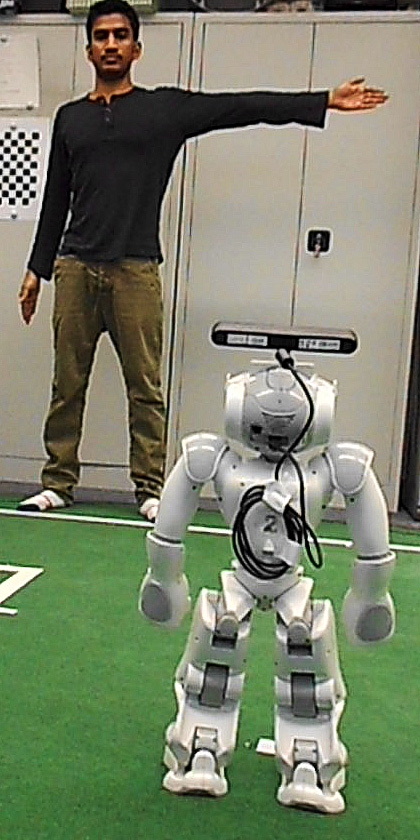
\includegraphics[height=95mm]{figures/result/usr-move-left.jpg} \caption*{} 
	\end{minipage}
	\begin{minipage}
		{1 
		\textwidth} \hspace{-5 mm} 
		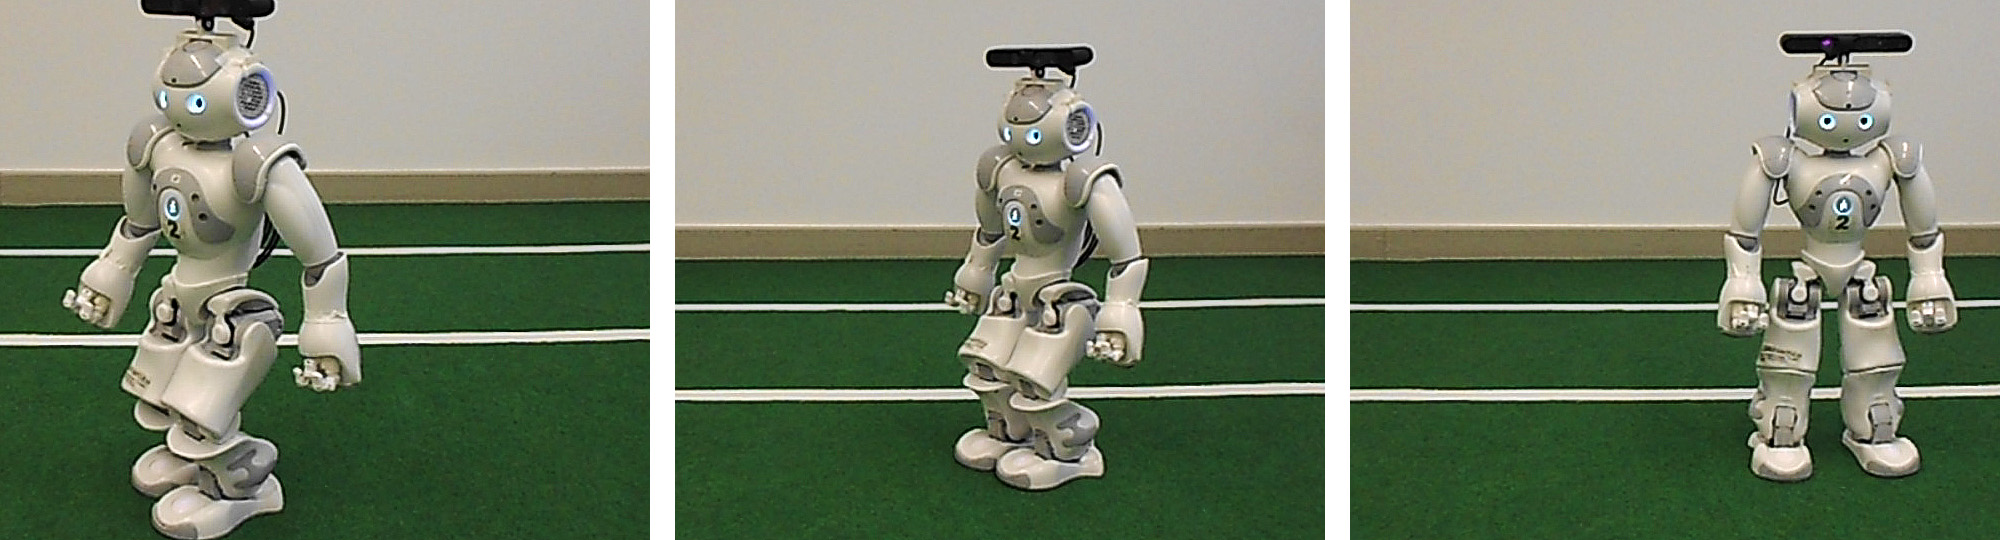
\includegraphics[width=160mm]{figures/result/nao-gm-move-left.jpg} 
	\end{minipage}
	\caption{NAO recognizes Move Left gesture and executes a predefined Gesture-To-Motion task.} \label{res:gm:move:left} 
\end{figure}
\begin{figure}
	[h] \hspace{-15 mm} \centering 
	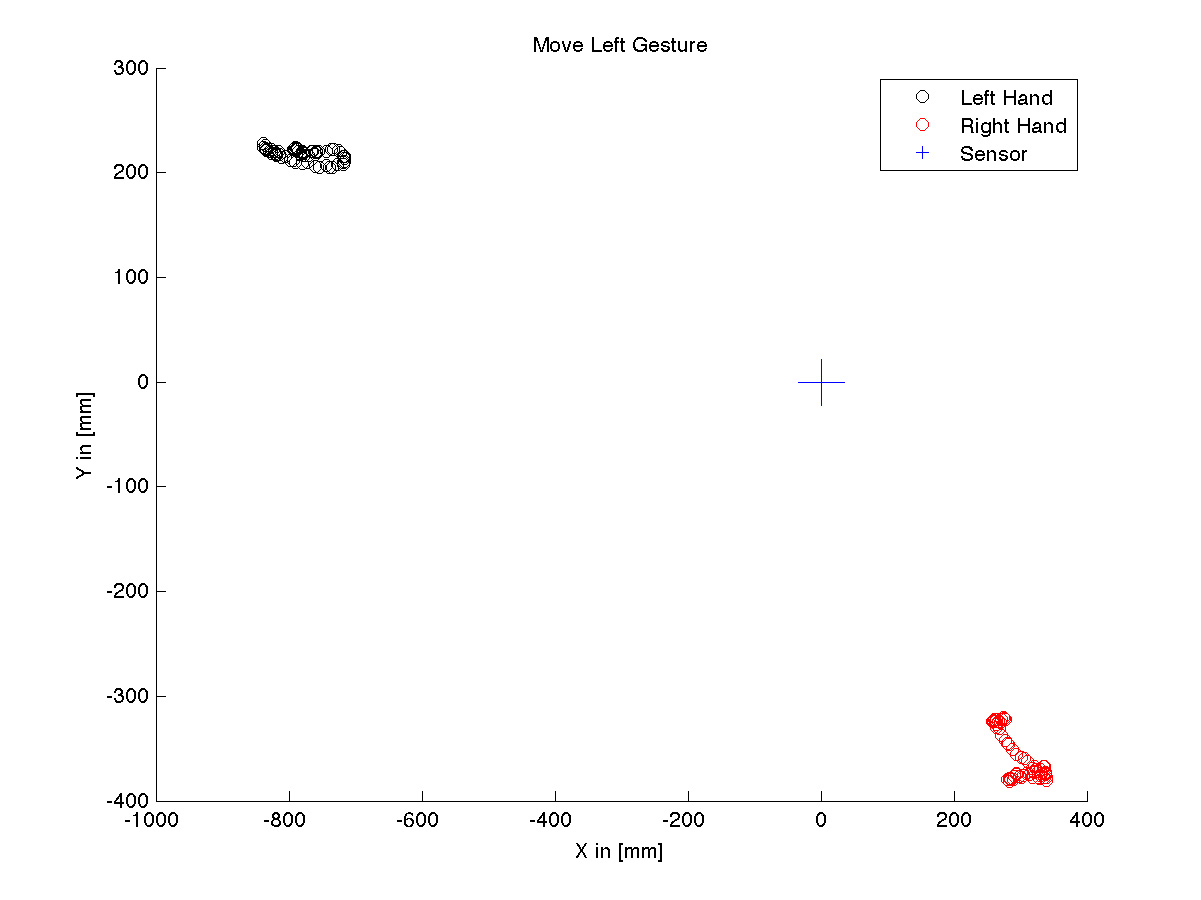
\includegraphics[width=155mm]{figures/result/test-move-left.jpg} \caption{Our system is capable of real time prediction by processing 30 samples per second. However, the detected hand gesture is triggered only when it is gesticulated for 1 second because of the post-processing by Class Label Filter module. The graph shows 60 samples of correctly recognized Move Left gesture. } \label{res:pl:move:left} 
\end{figure}
\begin{figure}
	[h] \centering 
	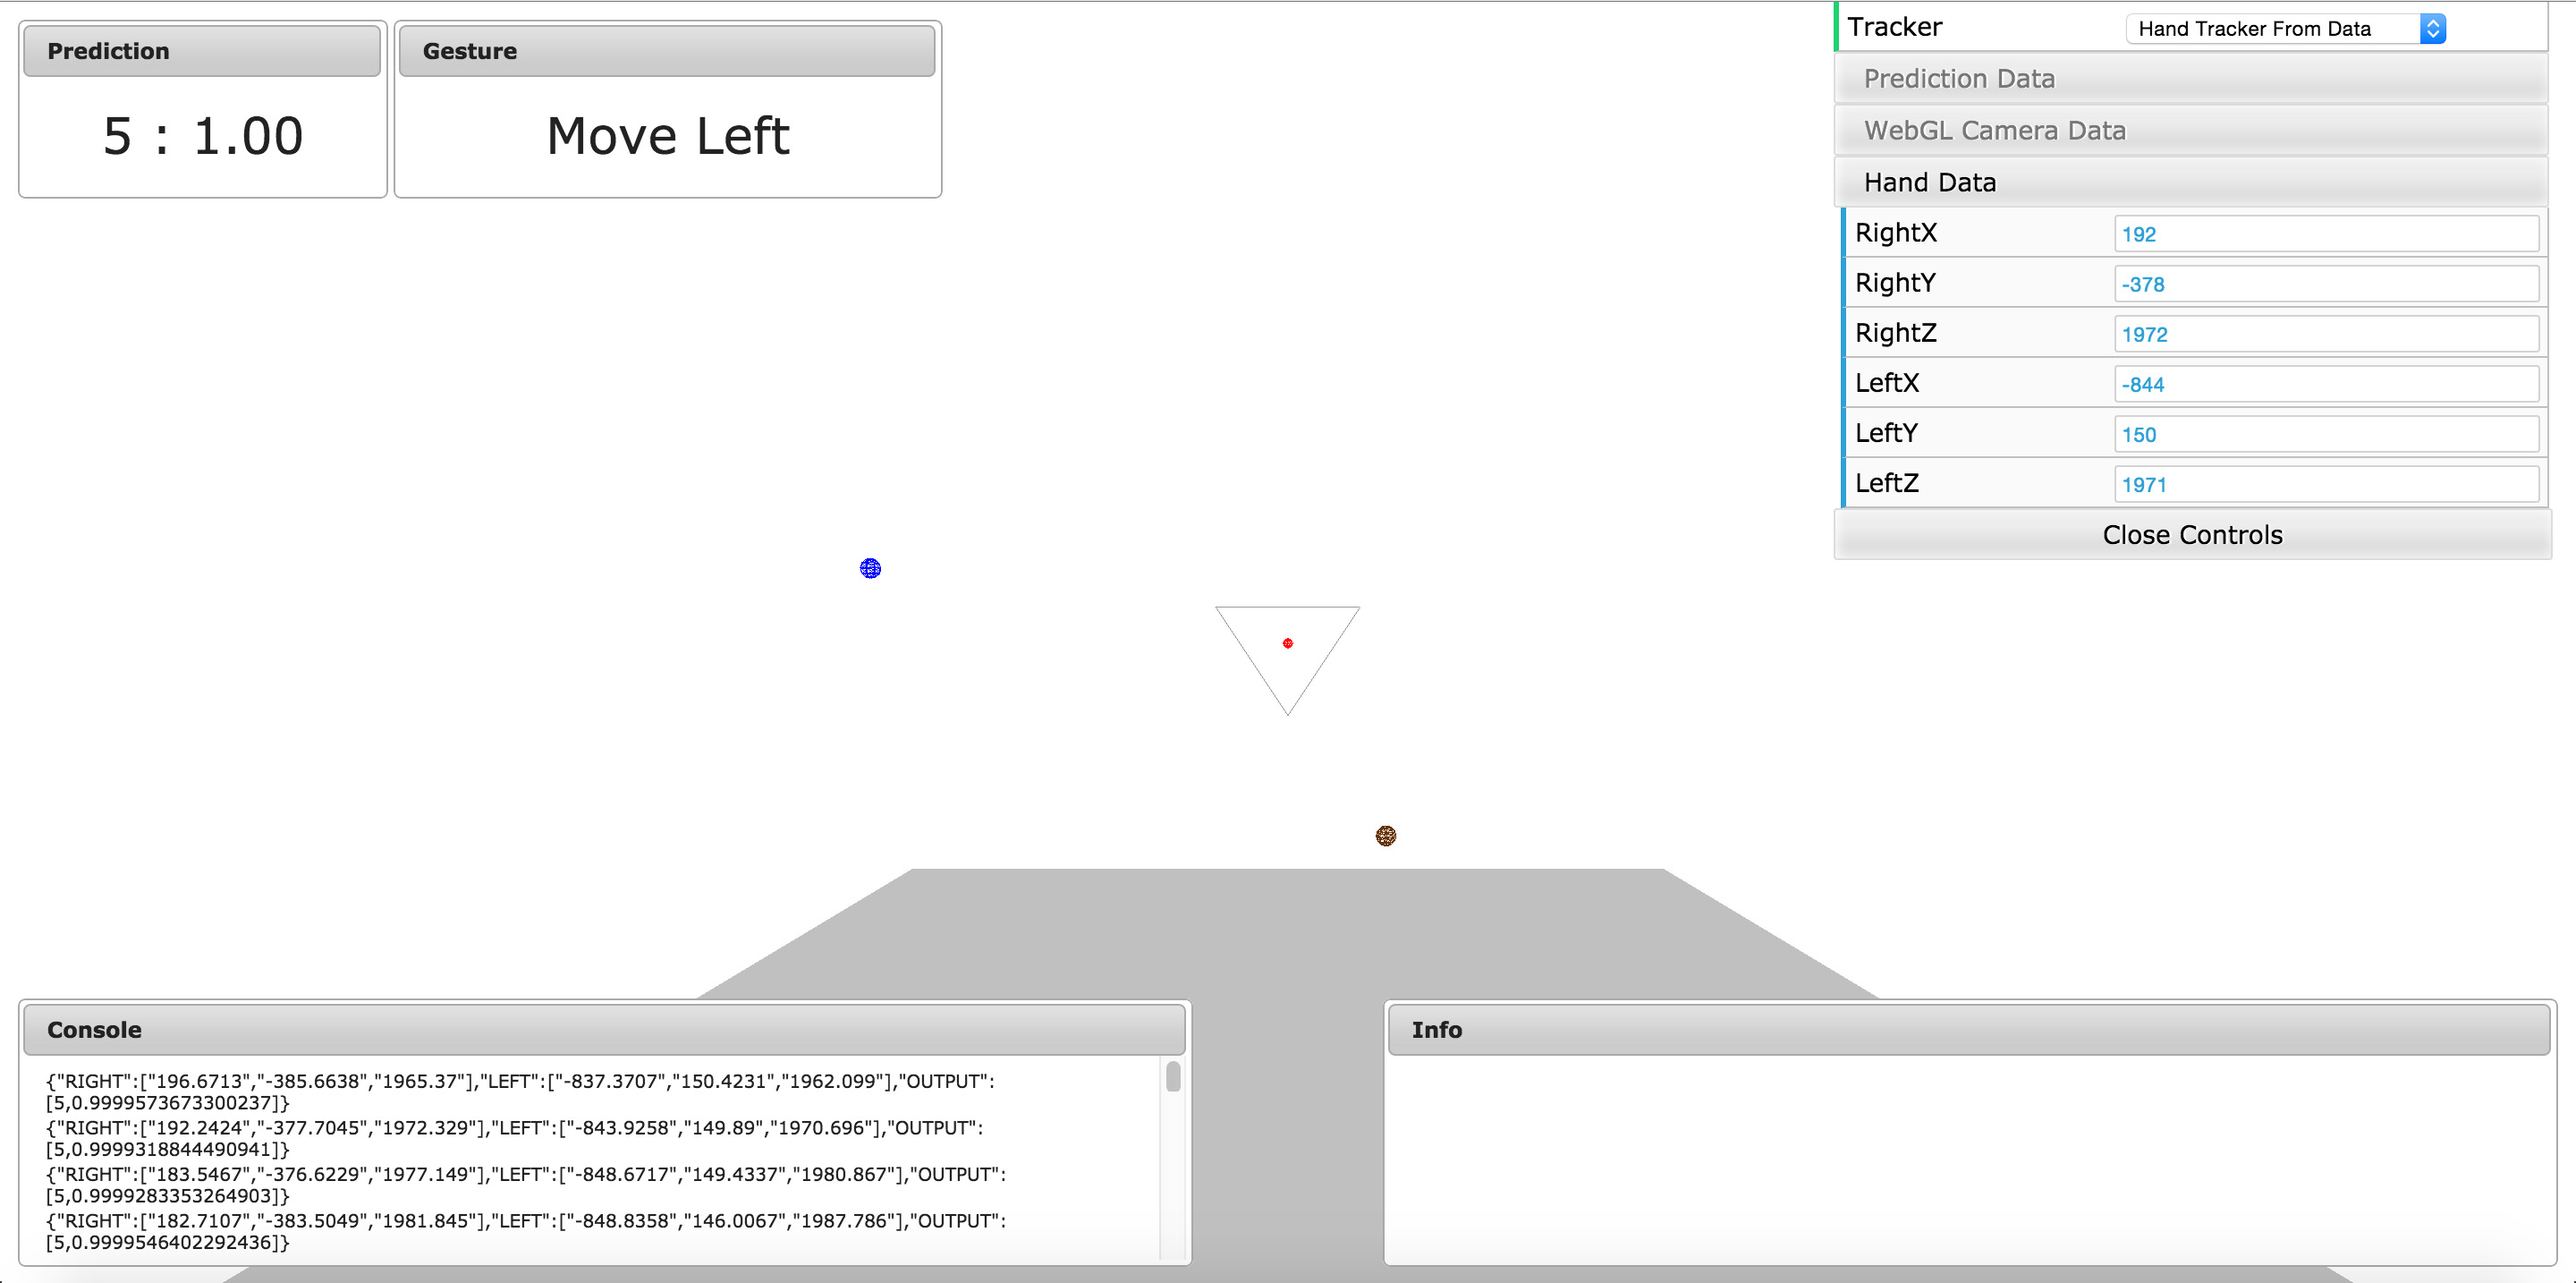
\includegraphics[height=70mm]{figures/result/cc-move-left.jpg} \caption{Control Center displays the recognized Move Left gesture in real time with the positions of left and left hand in 3 dimensional space.} \label{res:cc:move:left} 
\end{figure}
